\chapter{Giải tích}

\begin{figure}[ht]
    \centering
    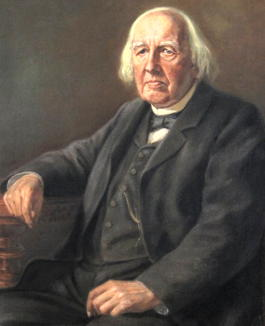
\includegraphics{mathematicians/Weiertrass.jpg}
    \captionsetup{labelformat=empty}
    \caption{Karl Theodor Wilhelm Weierstrass (1815-1897)}
\end{figure}

\section{Giới hạn}

\subsection*{Giới hạn của dãy số}

\begin{definition}[Giới hạn hữu hạn của dãy số]
    Cho dãy số $\{ a_n \}$. Ta nói dãy $\{ a_n \}$ có giới hạn hữu hạn $L$ nếu với mọi $\varepsilon > 0$, tồn tại $n_0 \in \NN$ sao cho với mọi $n \geqslant n_0$ thì 
    \begin{equation*}
        | a_{n} - L | < \varepsilon
    \end{equation*}

    Ký hiệu: $\displaystyle{\lim_{n \to \infty} a_n = L}$.
\end{definition}

\begin{example}
    Xét dãy số cho bởi công thức $a_n = \dfrac{1}{n}$. Ta chứng minh dãy số có giới hạn hữu hạn là 0.

    Với mọi $\varepsilon > 0$ tùy ý, ta cần chứng minh tồn tại số $n_0 \geqslant 1$ sao cho với mọi $n \geqslant n_0$ thì $| a_n - 0 | < \varepsilon$.

    Nói cách khác $a_{n_0} < \varepsilon$, hay tương đương với $\dfrac{1}{n_0} < \varepsilon \Leftrightarrow n_0 > \frac{1}{\varepsilon}$.

    Vậy ta chỉ cần chọn $n_0$ thỏa bất đẳng thức trên (luôn tìm được).

    Kết luận: $\displaystyle{\lim_{n \to \infty} a_n = 0}$
\end{example}

\begin{definition}[Dãy số có giới hạn vô cực]
    Cho dãy số $\{a_n\}$. Ta nói dãy số có giới hạn ở dương vô cực nếu với mọi $M > 0$, tồn tại $n_0 \in \NN$ sao cho với mọi $n \geqslant n_0$ thì $a_n > M$.
\end{definition}

Nói cách khác, nếu ta chọn một số $M$ rất lớn bất kì, thì mọi số hạng của dãy số kể từ một số hạng nào đó trở đi luôn lớn hơn $M$. Định nghĩa về dãy số có giới hạn ở âm vô cực cũng tương tự.

\subsection*{Giới hạn của hàm số}

Để định nghĩa giới hạn của hàm số $y = f(x)$ khi $x$ tiến tới $x_0$ ta có hai loại định nghĩa.

\begin{definition}[Giới hạn hàm số qua giới hạn dãy số]
    Xét hàm số $f(x)$. Ta nói hàm số có giới hạn hữu hạn $L$ khi $x$ tiến tới $x_0$, nếu với mọi dãy số $\{x_n\}$ mà $\displaystyle{\lim_{n \to \infty} x_n = x_0}$, thì  $\displaystyle{\lim_{n \to \infty} f(x_n) = L}$.
\end{definition}

Định nghĩa này tuân theo giới hạn của dãy số. Khi đó mọi phần tử của dãy số từ một số hạng nào đó trở đi cho giá trị $f(x_n)$ tiến về $L$.

Định nghĩa của hàm số theo kiểu Cauchy (hay còn được gọi là ngôn ngữ $\delta-\varepsilon$) là kiểu định nghĩa phổ biến được giảng dạy trong nhà trường.

\begin{definition}[Giới hạn hàm số kiểu Cauchy]
    Xét hàm số $f(x)$. Ta nói hàm số có giới hạn hữu hạn $L$ khi $x$ tiến tới $x_0$, nếu với mọi $\varepsilon > 0$, tồn tại  $\delta > 0$ sao cho với mọi $x$ mà $| x - x_0 | < \delta$ thì $|f(x) - L| < \varepsilon$.

    Ký hiệu: $\displaystyle{\lim_{x \to x_0} f(x) = L}$
\end{definition}

%Một cách hình ảnh, tương tự như giới hạn dãy số, lần này ta nhìn trên 2 trục  của mặt phẳng tọa độ $Oxy$. Với mọi quả cầu bán kính $\varepsilon$ tâm $L$ (dành cho $f(x)$) ta luôn chọn được quả cầu bán kính $\delta$ tâm $x_0$ (dành cho $x$). Lúc này khi $x$ nằm trong quả cầu tâm $x_0$ bán kính $\delta$ thì $f(x)$ tương ứng sẽ nằm trong quả cầu tâm $L$ bán kính $\varepsilon$.

Ta có thể thấy ở đây $x$ tiến về $x_0$ (khá giống định nghĩa giới hạn hàm số) và $f(x)$ tương ứng tiến về $L$.

Tương tự ta cũng có giới hạn hàm số ở vô cực.

\begin{definition}[Giới hạn hàm số ở vô cực]
    Với hàm số $f(x)$, ta nói hàm số có giới hạn tại dương vô cực khi $x$ tiến về $x_0$ nếu với mọi $M > 0$, tồn tại $\delta > 0$ sao cho với mọi $x$ mà $|x - x_0| < \delta$ thì $f(x) > M$.

    Ký hiệu: $\displaystyle{\lim_{x \to x_0} f(x) = +\infty}$.
\end{definition}

\begin{definition}[Giới hạn một bên]
    Ta nói hàm số $f(x)$ có giới hạn phải $L$ tại $x_0$ khi $x$ tiến về bên phải $x_0$ nếu với mọi $\varepsilon > 0$, tồn tại $\delta > 0$ sao cho với mọi $0 < x - x_0 < \delta$  thì $|f(x) - L| < \varepsilon$.

    Ký hiệu: $\displaystyle{\lim_{x \to x_0^+} f(x) = L}$
\end{definition}

Nghĩa là chúng ta chỉ xét giới hạn khi $x$ tiến tới $x_0$ từ bên phải $x > x_0$. Tương tự cho giới hạn trái.

Lưu ý rằng trong nhiều trường hợp, mặc dù cùng tiến tới $x_0$ nhưng giới hạn trái và giới hạn phải có thể không bằng nhau.

\begin{example}
    Xét hàm số $y = \frac{1}{x}$. Ta thấy hàm số không xác định tại $x = 0$, và giới hạn trái và phải khác nhau do \[\lim_{x \to 0^+} = +\infty, \quad \lim_{x \to 0^-} = -\infty\]
\end{example}

\subsection*{Tính liên tục của hàm số}

Cho hàm số $f(x)$ xác định trên miền $D$ và $x_0$ là một điểm thuộc $D$.

\begin{definition}[Hàm số liên tục tại một điểm]
    Ta nói hàm số $f(x)$ liên tục tại $x_0$ nếu \[\lim_{x \to x_0} f(x) = f(x_0)\]
\end{definition}

Định nghĩa tương tự cho liên tục trái và liên tục phải (ta lấy giới hạn một bên).

Như vậy, có 3 khả năng hàm số không liên tục tại một điểm.

\begin{enumerate}[noitemsep]
    \item Hàm số không xác định tại $x_0$
    \item Hàm số xác định tại $x_0$ nhưng giới hạn tại đó không bằng $f(x_0)$
    \item Giới hạn trái và giới hạn phải không bằng nhau
\end{enumerate}

Nếu hàm số không liên tục tại $x_0$ ta gọi hàm số bị \textbf{gián đoạn} tại $x_0$.

Nếu hàm số liên tục tại mọi điểm trên khoảng $(a, b)$ thì ta nói hàm số liên tục trên khoảng đó.

\section{Đạo hàm}

\begin{definition}[Đạo hàm]
    Cho hàm số $f(x)$ xác định trên miền $D$ và $x_0$ là điểm thuộc $D$. Ta nói hàm số $f(x)$ có đạo hàm tại $x_0$ (hoặc khả vi tại $x_0$) nếu tồn tại giới hạn hữu hạn
    \[\lim_{x \to x_0}\frac{f(x) - f(x_0)}{x - x_0}\]

    Ký hiệu đạo hàm của $f$ tại $x_0$ là $f'(x_0)$.
\end{definition}

\begin{example}
    Xét hàm số $f(x) = x^2 + 1$ trên $\RR$. Tìm đạo hàm tại $x_0 \in \RR$.

    Ta có $f(x)-f(x_0) = x^2 + 1 - (x_0^2 + 1) = (x - x_0) (x + x_0)$.

    Khi đó $\frac{f(x)-f(x_0)}{x-x_0} = x + x_0$ nên ta có $\displaystyle{\lim_{x \to x_0} (x + x_0) = 2 x_0}$.
\end{example}

Nếu hàm số khả vi trên mọi điểm thuộc khoảng (đoạn) nào đó thì ta nói hàm số khả vi trên khoảng (đoạn) đó và ký hiệu là $f'(x)$.

Với ví dụ trên, ta thấy giới hạn tồn tại với mọi $x_0 \in \RR$ nên ta có thể thay $x_0$ bởi $x$ và có $f'(x) = 2x$ với $f(x) = x^2 + 1$.

\begin{remark}
    Từ định nghĩa ta thấy rằng nếu $f(x)$ khả vi tại $x_0$ thì nó cũng liên tục tại $x_0$. Tuy nhiên chiều ngược lại không đúng. Ví dụ với hàm số $y = \lvert x \rvert$, hàm số liên tục tại $x=0$ nhưng giới hạn (đạo hàm) phải là 1, còn giới hạn (đạo hàm) trái là -1.
\end{remark}

Về mặt hình ảnh, khi hàm số khả vi tại một điểm thì đồ thị sẽ "trơn", không gấp khúc tại điểm đó.

\subsection*{Cực trị}

Đầu tiên chúng ta cần một định lý về tính đơn điệu của hàm số
khả vi.

\begin{theorem}
    Xét hàm số $f(x)$ khả vi trên khoảng $(a, b)$. Nếu $f'(x) > 0$ 
    với mọi $x \in (a, b)$ thì $f(x)$ đồng biến trên $(a, b)$.
\end{theorem}

Tương tự, $f'(x) < 0$ với mọi $x \in (a, b)$ thì $f(x)$ nghịch biến trên
$(a, b)$.

\begin{definition}[Cực tiểu của hàm số]
    Xét hàm số $f(x)$ liên tục trên khoảng $(a, b)$. Điểm $(x_0, f(x_0))$ được
    gọi là \textbf{cực tiểu} của hàm số $f(x)$ nếu tồn tại một lân cận $U$
    chứa $x_0$ nằm trong khoảng $(a, b)$ sao cho với mọi $x \in U$ thì $f(x) \geqslant f(x_0)$.
\end{definition}

\begin{definition}[Cực đại của hàm số]
    Xét hàm số $f(x)$ liên tục trên khoảng $(a, b)$. Điểm $(x_0, f(x_0))$ được
    gọi là \textbf{cực đại} của hàm số $f(x)$ nếu tồn tại một lân cận $U$
    chứa $x_0$ nằm trong khoảng $(a, b)$ sao cho với mọi $x \in U$ thì $f(x) \leqslant f(x_0)$.
\end{definition}

Theo định nghĩa cực tiểu thì chỉ cần tồn tại lân cận chứa $x_0$
mà $f(x) \geqslant f(x_0)$ thì điểm đó là cực tiểu. Như vậy một hàm số có 
thể có nhiều cực tiểu, tương tự cũng có thể có nhiều cực đại.

Lưu ý rằng cực đại và cực tiểu không phải điểm chỉ giá trị lớn nhất
hay giá trị nhỏ nhất của hàm số. Nó chỉ lớn nhất hoặc nhỏ nhất trong
vùng lân cận đó theo định nghĩa, nên người ta còn gọi là cực trị địa phương.

%Xét hàm số $f(x)$ khả vi trên khoảng $(a, b)$. Gọi $f'(x)$ là
%đạo hàm của hàm số $f(x)$ trên $(a, b)$. Khi đó điểm $x_0 \in (a, b)$ được gọi là
%\begin{itemize}
 %   \item Cực tiểu nếu $f'(x)$ đổi chiều từ âm sang dương khi đi qua $x_0$
 %   \item Cực đại nếu $f'(x)$ đổi chiều từ dương sang âm khi đi qua $x_0$
%\end{itemize}

\begin{definition}[Dãy Cauchy]
    Dãy $(x_n)$ được gọi là dãy Cauchy nếu với mọi $\varepsilon > 0$, tồn tại $N_0 \in \NN$ sao cho, với mọi $m, n > N_0$ thì $\lvert x_m - x_n \rvert < \varepsilon$.
\end{definition}

\begin{theorem}[Tiêu chuẩn Cauchy]
    Dãy số $(x_n)$ có giới hạn hữu hạn khi và chỉ khi nó là dãy Cauchy.
\end{theorem}

\begin{theorem}[Bổ đề Fermat]
    Cho $f$ là một hàm số có đạo hàm trên $(a, b)$. Nếu $x_0 \in (a, b)$ là một điểm cực trị của $f$ thì ta có $f'(x_0) = 0$.
\end{theorem}

\begin{proof}
    Ta chứng minh trong trường hợp $x_0$ là điểm cực tiểu. Trường hợp điểm cực đại tương tự.

    Hàm $f$ có đạo hàm trên $(a, b)$ nên tại điểm $x_0$ nó có đạo hàm bên trái và đạo hàm bên phải, và hai đạo hàm này bằng nhau.

    Ta có $\displaystyle{f'(x_0^+) = \lim_{x \to x_0^+} \frac{f(x) - f(x_0)}{x - x_0}}$. Vì $x \to x_0^+$ nghĩa là $x > x_0$ ($x$ tiến tới $x_0$ từ bên phải), và do $x_0$ là cực tiểu $f(x) - f(x_0) \geqslant 0$ nên phân số dưới dấu giới hạn lớn hơn 0. Suy ra $f'(x_0^+) \geqslant 0$.

    Hoàn toàn tương tự ta chứng minh được $f'(x_0^-) \leqslant 0$. Và do $f'(x_0^+) = f'(x_0^-) = f'(x_0)$ nên $f'(x_0) = 0$.

    Ta có điều phải chứng minh.
\end{proof}

\begin{theorem}[Định lí Rolle]
    Xét hàm số $f$ liên tục trên đoạn $[a, b]$, có đạo hàm trên khoảng $(a, b)$ và $f(a) = f(b)$. Khi đó tồn tại $c$ thuộc $(a, b)$ sao cho $f'(c) = 0$.
\end{theorem}

\begin{theorem}[Định lí Lagrange]
    Xét hàm số $f$ liên tục trên đoạn $[a, b]$, có đạo hàm trên khoảng $(a, b)$. Khi đó tồn tại $c$ thuộc $(a, b)$ sao cho $f'(c) (b - a) = f(b) - f(a)$.
\end{theorem}

\begin{definition}[Hàm lõm]
    Hàm số $f$ liên tục trên khoảng $\II$ nếu với mọi $\alpha, \beta$ mà $\alpha + \beta = 1$ ta đều có 
    \begin{equation}
        f(\alpha x + \beta y) \leqslant \alpha f(x) + \beta f(y), \quad \forall x, y \in \II
    \end{equation}
\end{definition}